\documentclass[a4paper]{article}

%·······························································································
%                                _    _                _           
%                               | |  | |              | |          
%                               | |__| | ___  __ _  __| | ___ _ __ 
%                               |  __  |/ _ \/ _` |/ _` |/ _ \ '__|
%                               | |  | |  __/ (_| | (_| |  __/ |   
%                               |_|  |_|\___|\__,_|\__,_|\___|_|   
%·······························································································

% Packages import
\usepackage[spanish]{babel}     % Spanish language support
\usepackage[utf8]{inputenc}     % UTF-8 encoding
\usepackage[T1]{fontenc}        % Proper font encoding
\usepackage{geometry}           % Page layout
\usepackage{titlesec}           % Custom section titles
\usepackage{lmodern}            % Modern font
\usepackage{fancyhdr}           % Header and footer
\usepackage{graphicx}           % Inserting images
\usepackage{anyfontsize}        % Arbitrary font size
\usepackage{listings}           % Code formatting
\usepackage{caption}            % Caption customizing
\usepackage{float}              % Image placing
\usepackage{sourcesanspro}
\usepackage{array}
\usepackage[dvipsnames,x11names,table]{xcolor}
\usepackage[colorlinks=true,linkcolor=black,urlcolor=Emerald]{hyperref}

% Packages configurations {{{

    % Adjust margins
    \geometry{a4paper, margin=2.5cm}

    % Change font family
    \renewcommand{\familydefault}{\sfdefault}
    
    % Change default command to resize all text
    \renewcommand{\normalsize}{\fontsize{13}{16}\selectfont}

    % Change section size
    \titleformat{\section}
        {\fontsize{16}{16}\selectfont\bfseries}
        {\thesection}{1em}{}

    % Change subsection size
    \titleformat{\subsection}
        {\fontsize{14}{16}\selectfont\bfseries}
        {\thesubsection}{1em}{}

    % Change table's cells padding
    \setlength{\tabcolsep}{12pt}
    \renewcommand{\arraystretch}{1.5}
    
    % Header/Footer settings
    \fancyfoot[C]{\thepage}

    % Shell prompt code
    \lstdefinestyle{shellprompt}{
        backgroundcolor=\color{black},
        basicstyle=\fontsize{11}{20}\ttfamily\color{white},
        keywordstyle=\color{NavyBlue},
        commentstyle=\color{white},
        stringstyle=\color{green},
        breaklines=true,
    }

    % Define the style for code with line numbers
    \lstdefinestyle{normalcode}{
        numbers=left,         % Display line numbers on the left
        numberstyle=\tiny,    % Small size for the line numbers
        stepnumber=1,         % Number every line
        numbersep=5pt,        % Space between line numbers and code
        backgroundcolor=\color{lightgray}, % Background color of code block
        basicstyle=\ttfamily\footnotesize, % Set font to typewriter and small size
    }

    % Set default listings style to shellprompt
    \lstset{style=shellprompt}

% }}}

\hyphenpenalty=10000  % Avoid hyphenation
\exhyphenpenalty=10000
\sloppy  % Loosens the strictness of the justification algorithm
\newcommand{\textgap}{\vspace{1em}}

% Metadata {{{

    % Title
    \title{Sistemas Cooperativos y Gestión de Contenidos}
    
    % Author
    \author{Juan Manuel Segura Duarte}

% }}}













%·······························································································
%                     _____                                        _   
%                    |  __ \                                      | |  
%                    | |  | | ___   ___ _   _ _ __ ___   ___ _ __ | |_ 
%                    | |  | |/ _ \ / __| | | | '_ ` _ \ / _ \ '_ \| __|
%                    | |__| | (_) | (__| |_| | | | | | |  __/ | | | |_ 
%                    |_____/ \___/ \___|\__,_|_| |_| |_|\___|_| |_|\__|
%·······························································································
\begin{document}

% Cover Page
\begin{titlepage}
    \centering
    \vspace*{3cm}  % Space at the top
    {\Huge \textbf{SCGC Práctica 5}} % Custom title
    \vspace{1cm}
    
    {\Large Sistemas Cooperativos y Gestión de Contenidos: Desarrollo de la 5ª práctica} % Subtitle
    
    
\includegraphics[width=0.5\textwidth]{images/ugr-logo.png}
    \vspace{1cm}
    
    \textbf{\Large Juan Manuel Segura Duarte} % Author name
\end{titlepage}
\newpage

% Table of Contents page
\thispagestyle{empty}
\tableofcontents

%%%%%%%%%%%%%%%%%%%%%%%%%%%%%%%%%%%%%%%%%%%%%%%%%%%%%%%%%%%%%%%%%%%%%%%%%%%%%%%%%%%%%%%%%%%%%%%%%%
%%%%%%%%%%%%%%%%%%%%%%%%%%%%%%%%%%%%%%%%%%%%%%%%%%%%%%%%%%%%%%%%%%%%%%%%%%%%%%%%%%%%%%%%%%%%%%%%%%
%%%%%%%%%%%%%%%%%%%%%%%%%%%%%%%%%%%%%%%%%%%%%%%%%%%%%%%%%%%%%%%%%%%%%%%%%%%%%%%%%%%%%%%%%%%%%%%%%%

% Start numbering in this page (after the title page and index)
\newpage
\pagenumbering{arabic}
\setcounter{page}{1}


\section{Análisis de plugins}

Tras un análisis profundo de la página desarrollada se ha llegado a la conclusión de escoger estos 5 plugins en la parte primera de esta práctica:

\begin{itemize}
    \item Link Library (sección 5.7.3)
    \item Contact Form 7 (sección 5.7.9)
    \item MailPoet (sección 5.7.12)
    \item Spam protection AntiSpam, FireWall by CleanTalk (sección 5.7.13)
    \item WP Maintenance Mode (sección 5.7.14)
\end{itemize}


% plugin 1.1
\subsection{Contact Form 7 (Categoría: Formularios de contacto)}

\textbf{Análisis}
\begin{itemize}
    \item Descripción del plugin: Plugin líder para creación de formularios personalizables con gestión multi-formulario, soporte para campos dinámicos e integración con servicios de terceros.
    \item Valoración de los usuarios: 4/5 (2,129 valoraciones)
    \item Valoración profesional:
    \begin{itemize}
        \item Adaptación a la plantilla elegida: Compatibilidad total con temas modernos. Permite ajustar estilos CSS para armonizar con la identidad visual.
        \item Condiciones para su uso: Gratuito y \textit{privacy-friendly} por defecto.
    \end{itemize}
\end{itemize}

\textbf{Funcionalidad añadida:} Creación de formularios personalizados para:
\begin{itemize}
    \item Pedidos especiales (ej: algún producto que no esté en el catálogo).
    \item Consultas sobre disponibilidad de productos (ej: "¿Tienen chuletón de buey?").
\end{itemize}


\textbf{Justificación del aporte:}
\begin{itemize}
    \item Problema resuelto: Antes, los clientes solo podían contactar por teléfono, lo que generaba saturación en horas punta, o por correo electrónico, el cual no es un sistema tan frecuentemente usado como para poder sustituir al teléfono.
    \item Impacto en la web: Ahora los clientes tienen una forma cómoda de hacer preguntas, sin tener que estar pendientes de ver cuándo pueden llamar o refrescando el correo para ver si le han respondido.
\end{itemize}


\textbf{Justificación de la elección frente a las alternativas:}
\begin{itemize}
    \item Razón principal: Contact Form 7 tiene más de 10 millones de instalaciones activas frente a WPForms Lite, en la imagen adjunta se puede ver como es la primera opción que aparece cuando buscas ``contact form'' en el catálogo de plugins de WordPress, con una media de 4 estrellas y más de 2000 valoraciones, lo que parece indicar se trata de un plugin respetado por la comunidad.
    \item Ventaja clave: Es completamente gratuito, por lo que no es necesario aumentar el coste de la web.
\end{itemize}

\begin{figure}[H]
    \centering
    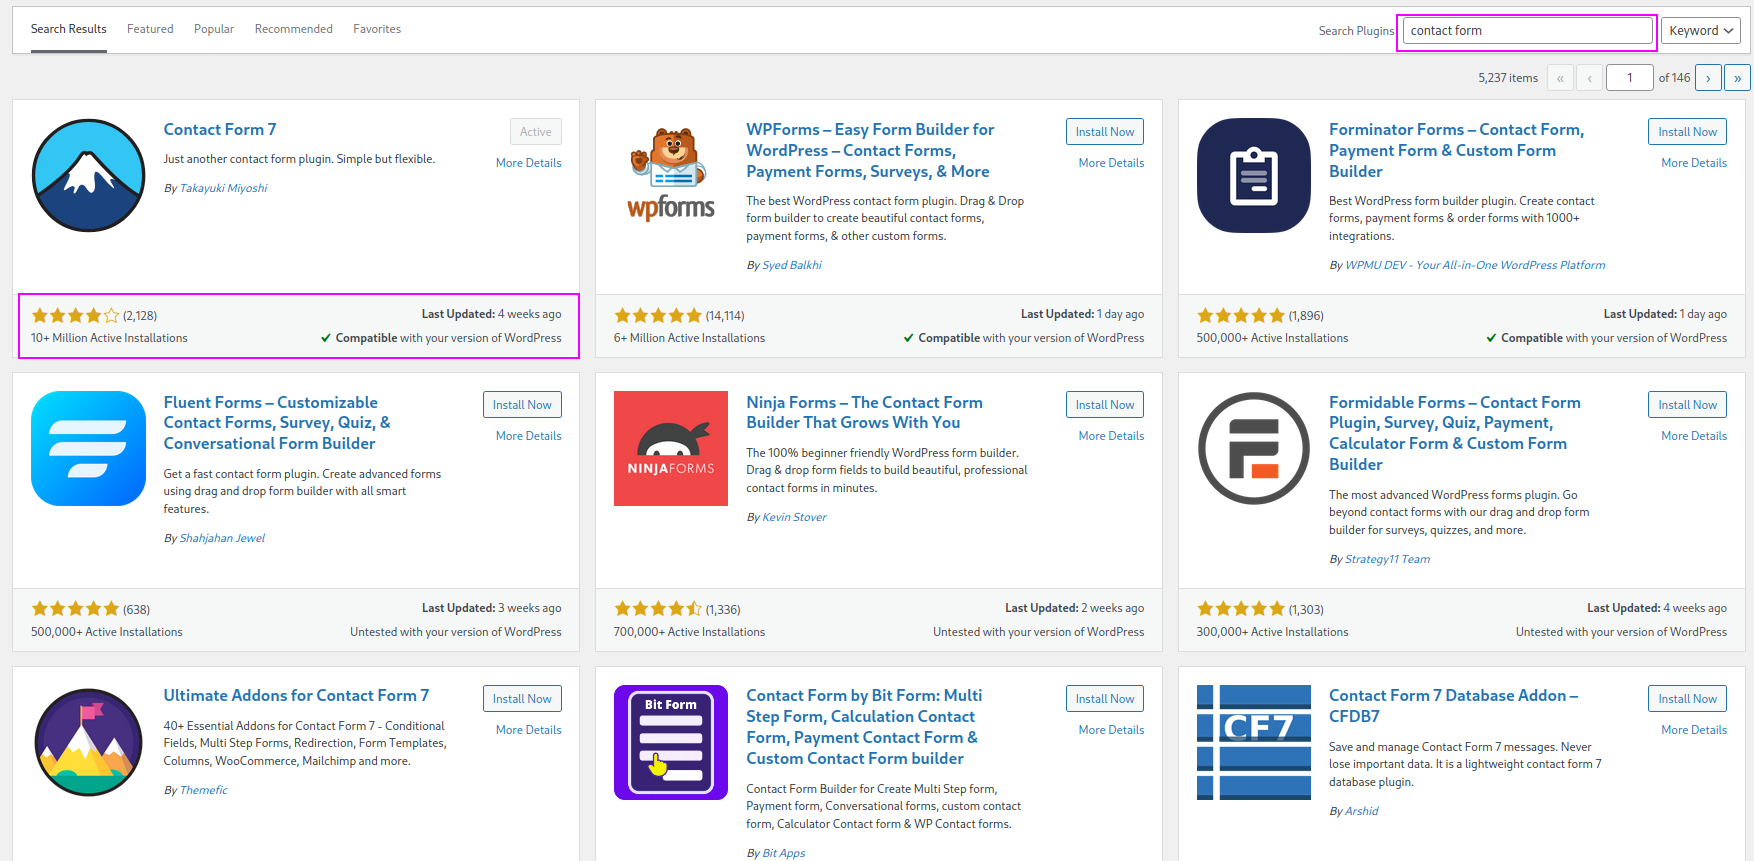
\includegraphics[width=0.85\textwidth]{images/popularidad-contact-form-7.png}
    \caption{Contact Form 7, primer resultado  de la búsqueda ``contact form'' en WP}
\end{figure}


% plugin 1.2
\subsection{WP Maintenance Mode (Categoría: Mantenimiento)}

\textbf{Análisis}
\begin{itemize}
    \item Descripción del plugin: Solución ligera para mostrar páginas de mantenimiento/coming soon con temporizador, suscripción por email y diseño responsive.
    \item Valoración de los usuarios: 4.5/5 (838 valoraciones)
    \item Valoración profesional:
    \begin{itemize}
        \item Adaptación a la plantilla elegida: Permite modificar la página de mantenimiento para que se ajuste al tema usado.
        \item Condiciones para su uso: Gratuito.
    \end{itemize}
\end{itemize}

\textbf{Funcionalidad añadida:} Página temporal de mantenimiento con:
\begin{itemize}
    \item Mensaje personalizado para notificar al cliente que alguna página no se encuentra disponible y alternativas como el número de teléfono.
    \item Countdown para reactivación (ej: "Volvemos en 2 horas").
\end{itemize}


\textbf{Justificación del aporte:}
\begin{itemize}
    \item Problema resuelto: Durante actualizaciones técnicas, los clientes veían errores o páginas incompletas, lo que generaba desconfianza.
    \item Impacto en la web: Mantiene la imagen profesional y comunica claramente que la carnicería sigue operativa físicamente.
\end{itemize}


\textbf{Justificación de la elección frente a las alternativas:}
\begin{itemize}
    \item Razón principal: WP Maintenance mode se centra en justo eso, a diferencia de Coming Soon Page \& Maintenance Mode, que ahora se llama ``Website Builder by SeedProd — Theme Builder, Landing Page Builder, Coming Soon Page, Maintenance Mode'', lo que da a entender que su ámbito se ha ampliado y ofrece más funcionalidades. Esto no es malo en sí pero más componentes implica mayor probabilidad de ruptura y teniendo en cuenta que no se necesitan ninguna de las otras funciones este plugin sería demasiado. Tampoco se ha escogido Maintenance Mode for Your Website porque, aunque sea el más popular, su estilo simplista que aún así aprovecha para establecer versions pagadas inspira desconfianza en lo personal. Por último no se ha utilizado Minimal Coming Soon \& Maintenance Mode porque tiene considerablemente menos instalaciones activas que el elegido, con +100,000 frente a +600,000, y una diferencia de solo 0.1 estrellas.
    \item Ventaja clave: Es completamente gratuito, por lo que no es necesario aumentar el coste de la web.
\end{itemize}

\begin{figure}[H]
    \centering
    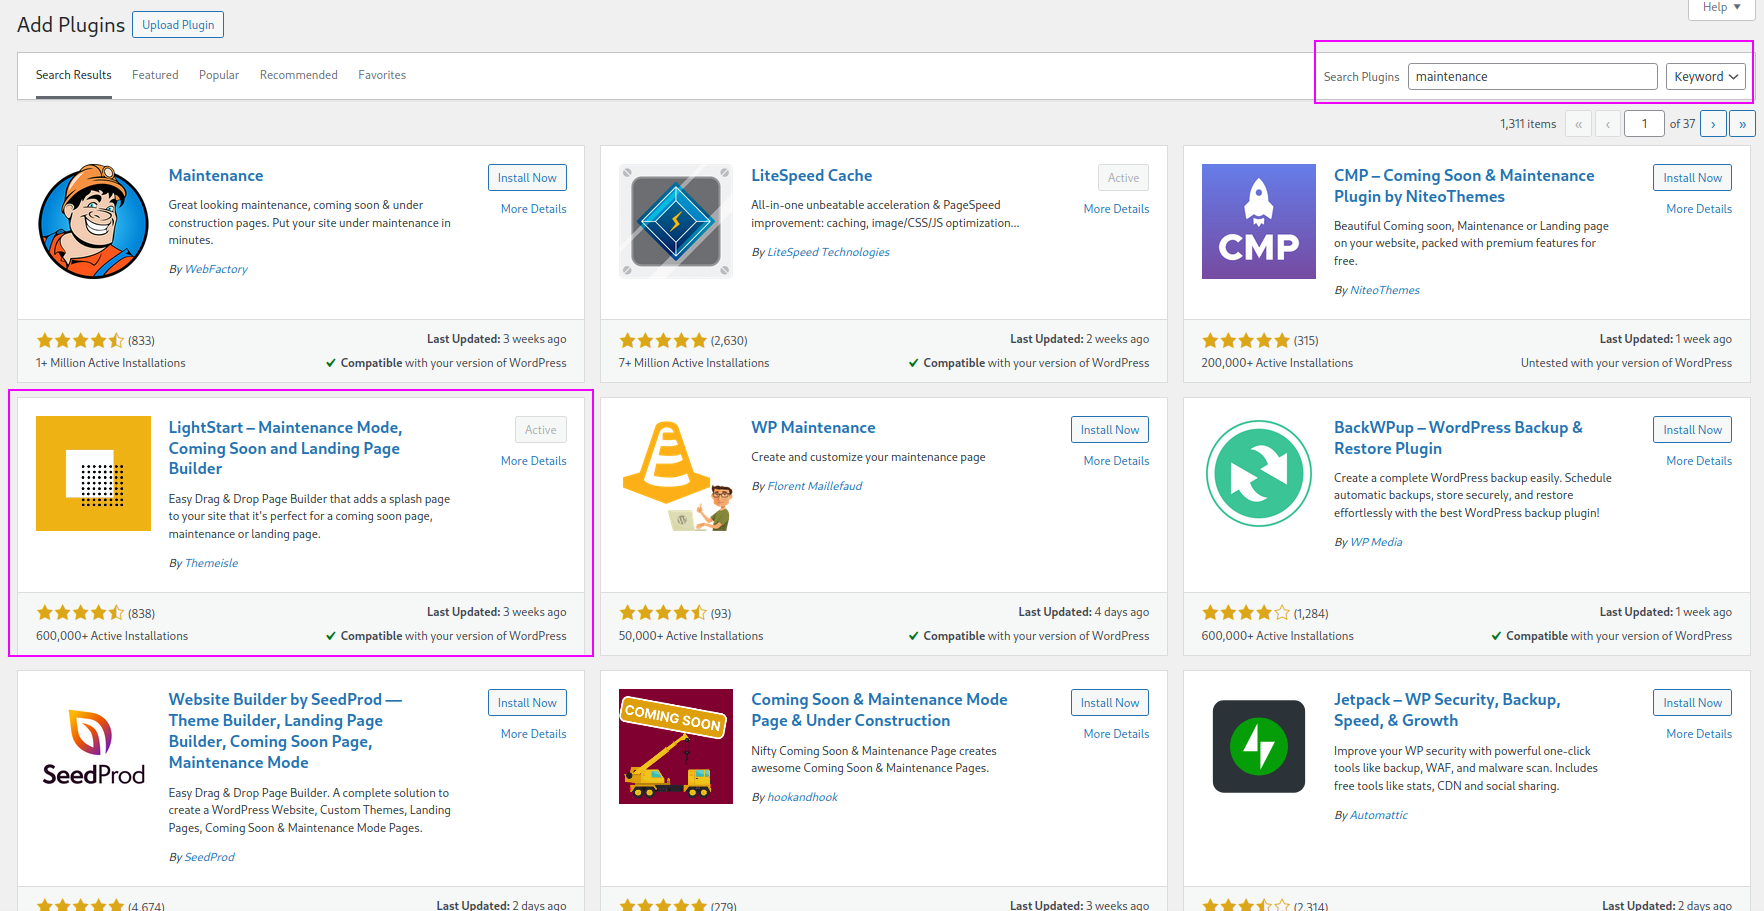
\includegraphics[width=0.85\textwidth]{images/popularidad-maintenance-mode.png}
    \caption{WP Maintenance Mode, solo por detrás de ``Maintenance''}
\end{figure}


% plugin 1.3
\subsection{Spam protection, AntiSpam, FireWall by CleanTalk (Categoría: Antispam)}

\textbf{Análisis}
\begin{itemize}
    \item Descripción del plugin: Suite de seguridad todo-en-uno con protección en tiempo real contra spam (comentarios, formularios, registros) mediante análisis en la nube y \textit{blacklist} automatizada. Incluye firewall básico.
    \item Valoración de los usuarios: 5/5 (3,061 valoraciones)
    \item Valoración profesional:
    \begin{itemize}
        \item Adaptación a la plantilla elegida: Agnóstico / sin relación con el frontend.
        \item Condiciones para su uso: Suscripción de pago obligatoriamente con prueba gratuita de 7 días.
    \end{itemize}
\end{itemize}

\textbf{Funcionalidad añadida:} Bloqueo automático de:
\begin{itemize}
    \item Comentarios falsos en posts de ``Ofertas'' (ej: ``¡Carnes a 1€! [enlace malicioso]'').
    \item Spam en formularios de contacto.
\end{itemize}


\textbf{Justificación del aporte:} 

Protege la reputación de la carnicería y evita que los clientes encuentren contenido no deseado.


\textbf{Justificación de la elección frente a las alternativas:}
\begin{itemize}
    \item Razón principal: Es el plugin más famoso, con mejores valoraciones, que no se centra solo en los formularios de Contact Form 7 (a diferencia de Honeypot) y que sigue estando mantenido (a diferencia de WPBruiser, que se actualizó por última vez hace 5 años).
    \item Ventajas: Gran cantidad de características para eliminar contenido no deseado.
\end{itemize}

\begin{figure}[H]
    \centering
    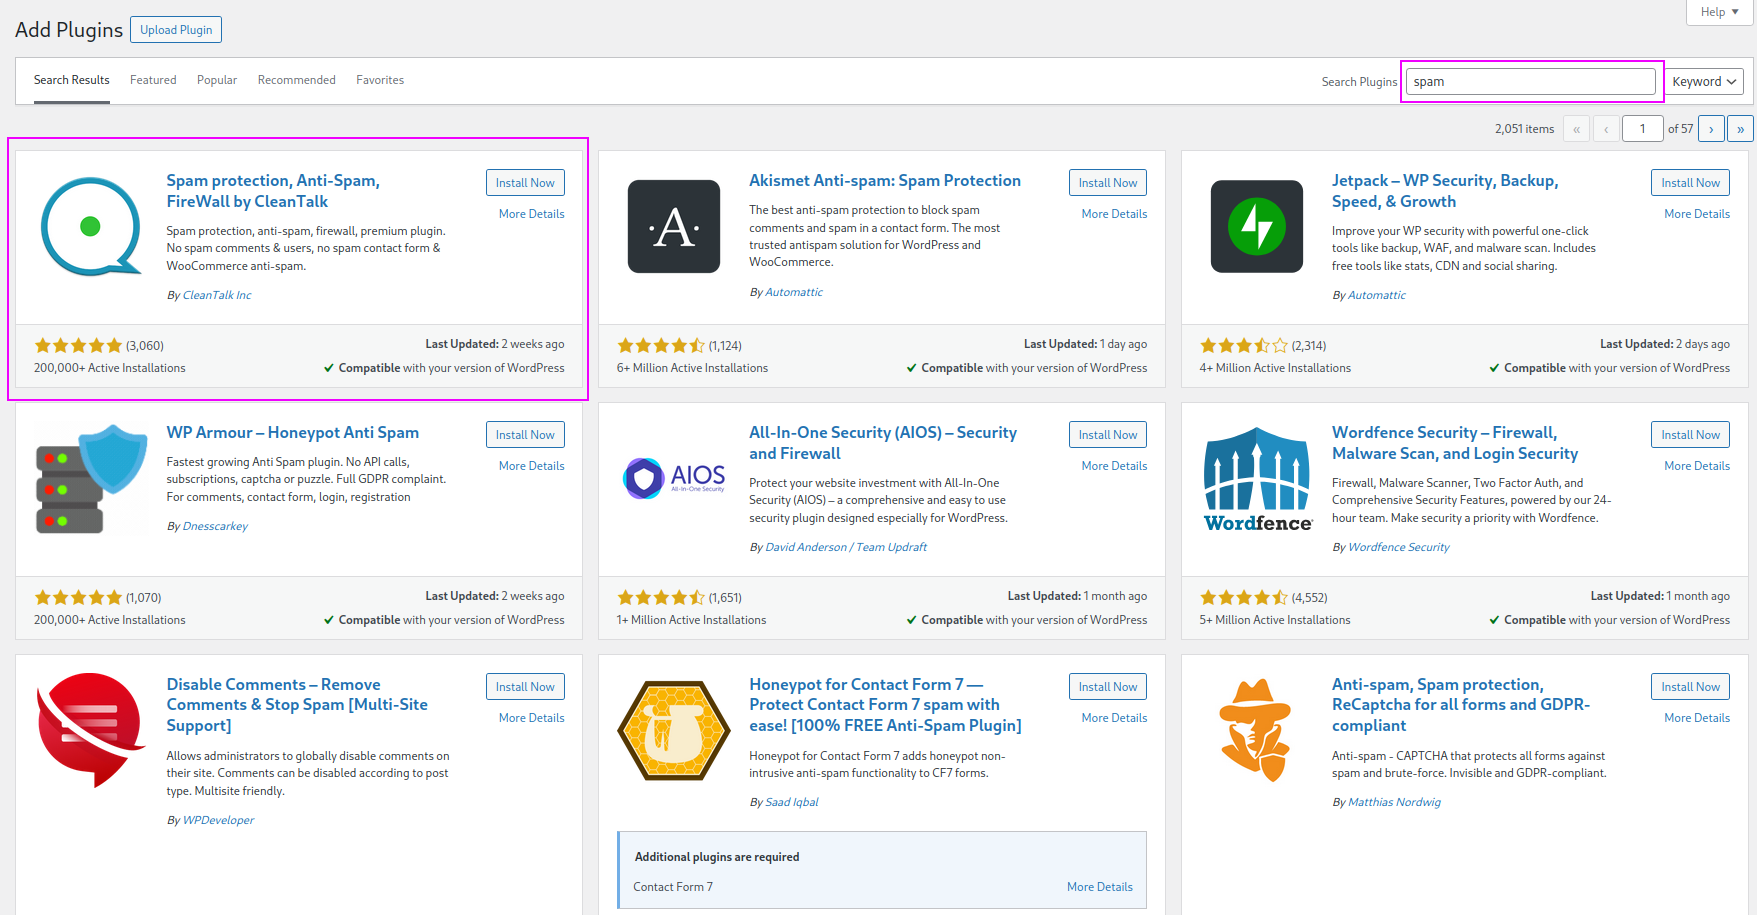
\includegraphics[width=0.85\textwidth]{images/popularidad-antispam.png}
    \caption{Spam protection, AntiSpam, FireWall by CleanTalk}
\end{figure}


% plugin 1.4
\subsection{MailPoet (Categoría: Newsletter)}

\textbf{Análisis}
\begin{itemize}
    \item Descripción del plugin: Sistema completo de email marketing integrado con WordPress. Permite creación de newsletters con gestión de suscriptores y análisis básicos.
    \item Valoración de los usuarios: 4.5/5 (1,375 valoraciones)
    \item Valoración profesional:
    \begin{itemize}
        \item Adaptación a la plantilla elegida: Ofrece plantillas responsive editables.
        \item Condiciones para su uso: Requiere configuración SMTP para entregabilidad óptima. Deben implementarse formularios de doble opt-in para cumplir con GDPR.
    \end{itemize}
\end{itemize}

\textbf{Funcionalidad añadida:} Envío de newsletters con:
\begin{itemize}
    \item Ofertas semanales (ej: ``Chorizos artesanales al 15\% de descuento'').
    \item Recetas exclusivas (ej: ``Cómo preparar un asado perfecto en 5 pasos'').
\end{itemize}

\textbf{Justificación del aporte:}
\begin{itemize}
    \item Problema resuelto: Los clientes no tenían forma de recibir actualizaciones sin revisar manualmente la web.
    \item Impacto en la web: Es probable que aumente las ventas debido a la facilidad para recibir todo tipo de ofertas.
\end{itemize}
    

\textbf{Justificación de la elección frente a las alternativas:}
\begin{itemize}
    \item Newsletter: Requiere conocimientos técnicos para personalizar plantillas.
    \item Mailchimp for WP: Necesita cuenta externa (MailChimp).
\end{itemize}

\begin{figure}[H]
    \centering
    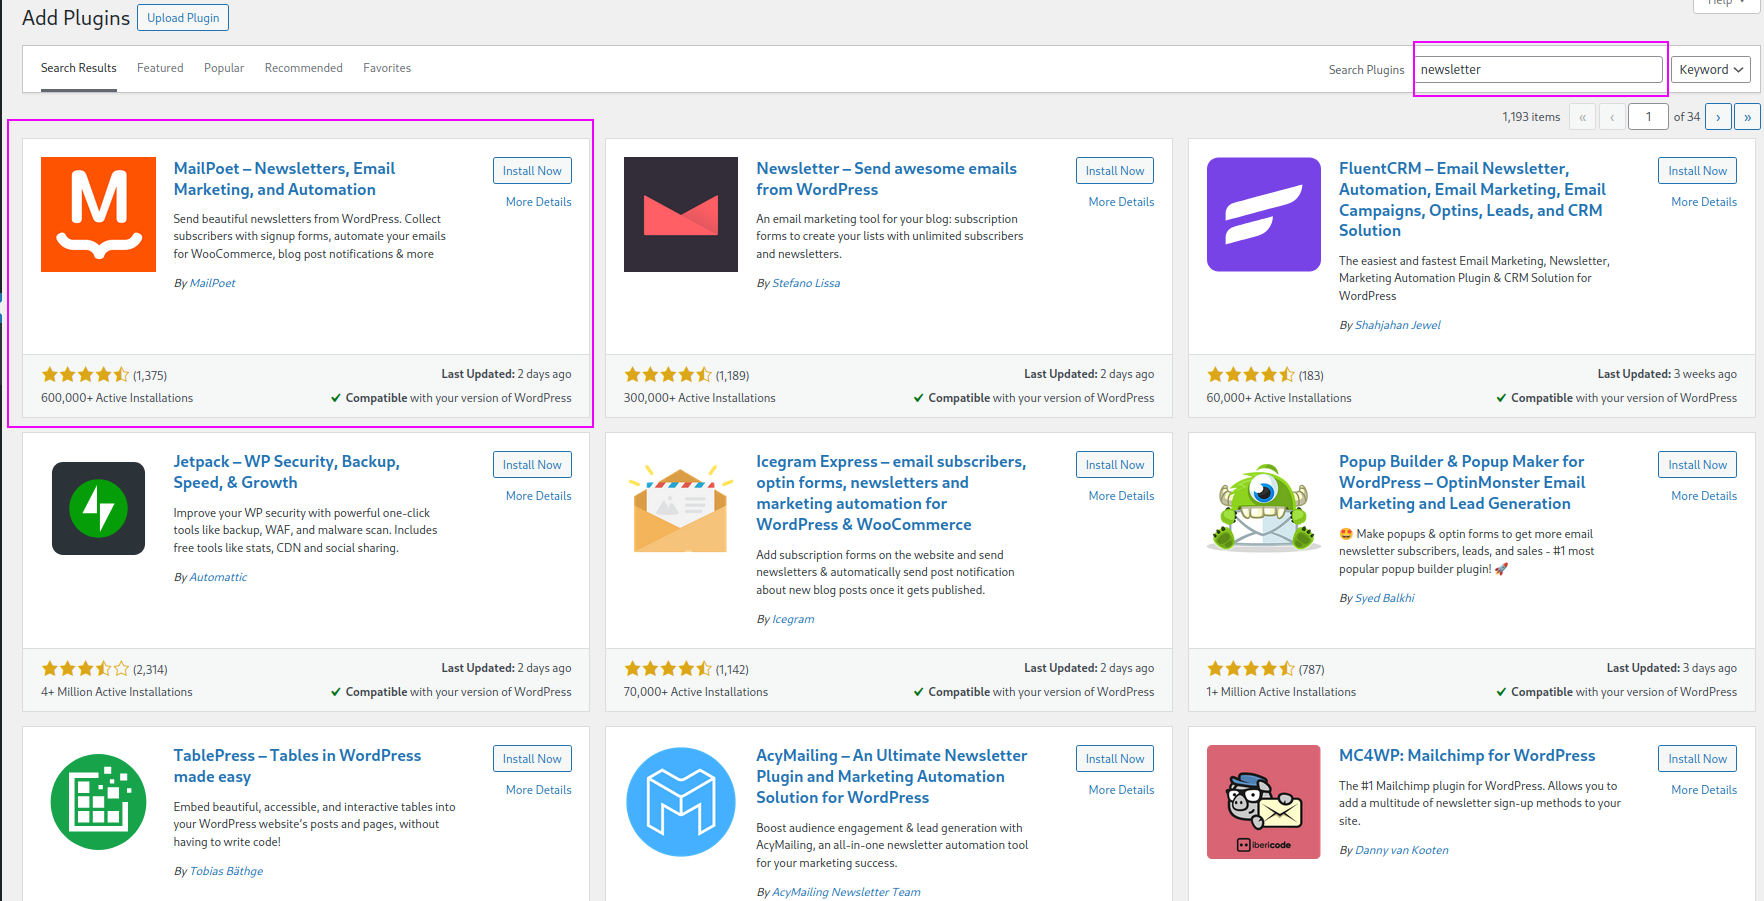
\includegraphics[width=0.85\textwidth]{images/popularidad-mailpoet.png}
    \caption{MailPoet, primer resultado al buscar ``newsletter''}
\end{figure}


% plugin 1.5
\subsection{Link Library (Categoría: Repositorio de enlaces)}

\textbf{Análisis}
\begin{itemize}
    \item Descripción del plugin: Gestor avanzado de enlaces externos con soporte para categorización múltiple, vistas personalizadas (grid/listado) y sistema de votación.
    \item Valoración de los usuarios: 4.5/5 (96 votos)
    \item Valoración profesional:
    \begin{itemize}
        \item Adaptación a la plantilla elegida: Permite generar shortcodes con estilos específicos que se integran fluidamente en cualquier página.
        \item Condiciones para su uso: Gratuito.
    \end{itemize}
\end{itemize}

\textbf{Funcionalidad añadida:} Directorio público de recursos gratuitos:
\begin{itemize}
    \item Libros PDF sobre cortes de carne (ej: "Guía del Carnicero Moderno").
    \item Enlaces a recetas de chefs reconocidos.
\end{itemize}


\textbf{Justificación del aporte:}
\begin{itemize}
    \item Los clientes buscaban ideas para cocinar, pero la web no ofrecía valor educativo.
\end{itemize}


\textbf{Justificación de la elección frente a las alternativas:}
\begin{itemize}
    \item Gallery Custom Links: Solo permite enlaces en galerías de imágenes, no en listados organizados. Última vez que se actualizó fue hace 4 meses, mientras que Link Library se actualizó hace 3 semanas.
    \item Huge-IT Portfolio Gallery: Desabilitado desde el 7 de febrero de 2018 por violación de las normas, según WordPress.
\end{itemize}

\begin{figure}[H]
    \centering
    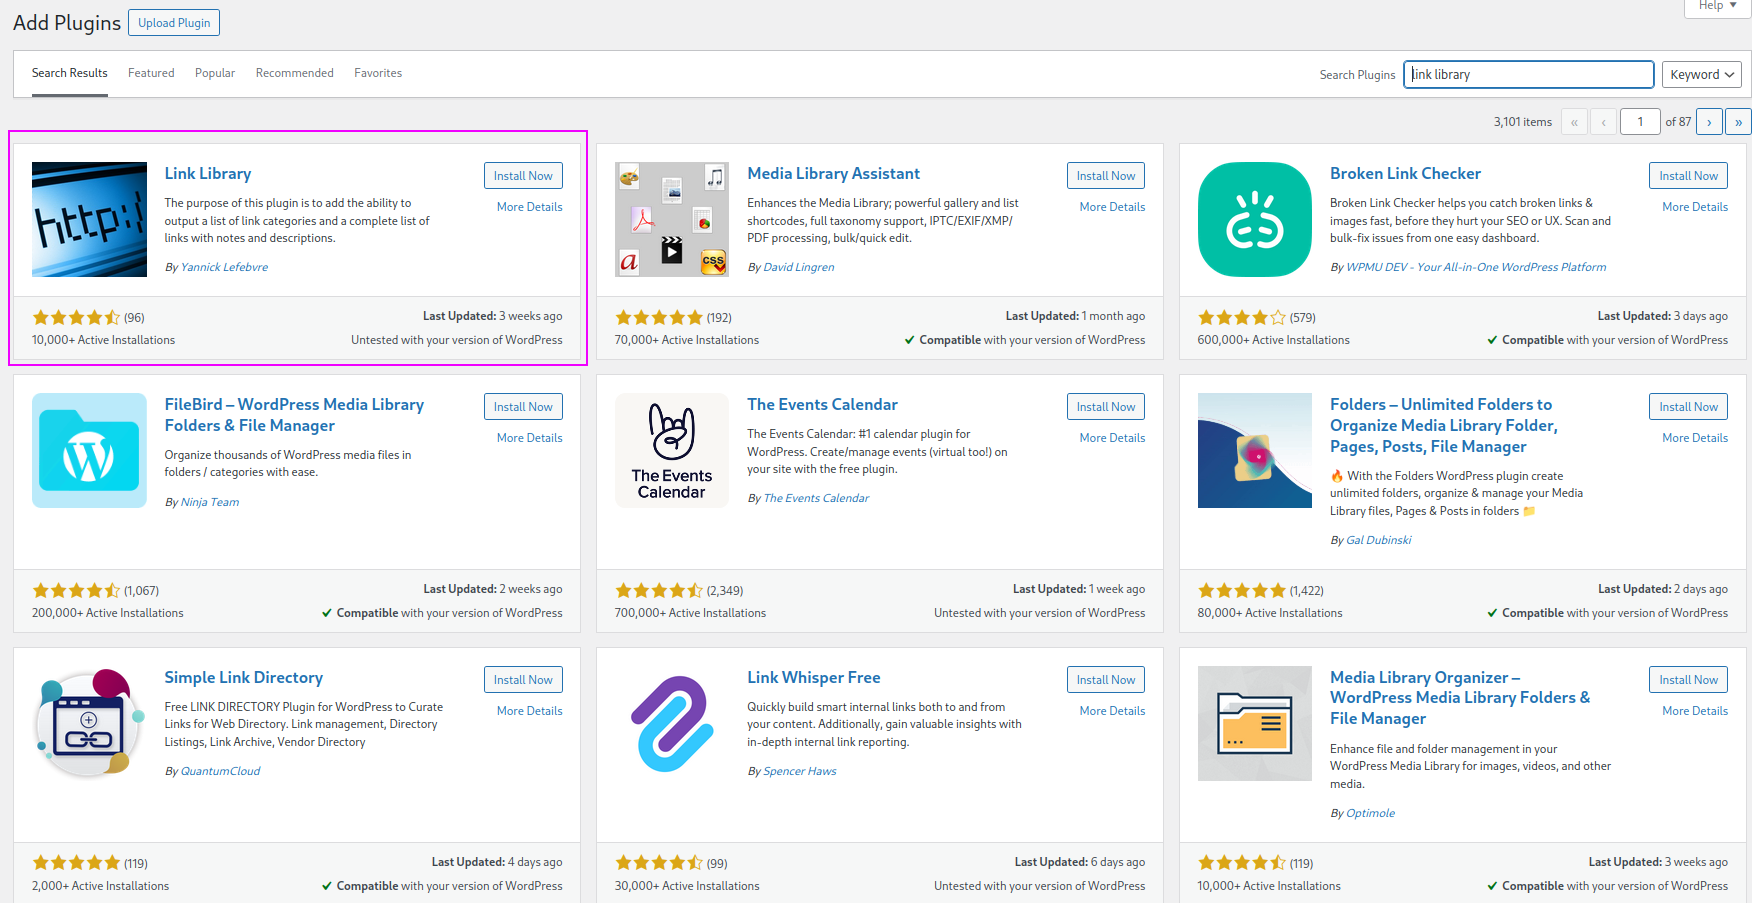
\includegraphics[width=0.85\textwidth]{images/popularidad-link-library.png}
    \caption{Link Library en el marketplace de plugins de WordPress}
\end{figure}

\newpage



\section{Creación de un widget para wordpress}

\subsection{Preámbulo}

Los temas de bloques en WordPress (como el utilizado en esta práctica) representan una evolución técnica donde los widgets clásicos han sido reemplazados por bloques y partes de plantilla. A continuación, se explica la aparente contradicción de que el tema incluya la etiqueta "footer widgets" sin usar widgets tradicionales:

\begin{enumerate}
    \item Transición técnica

        Widgets vs. Bloques:

        \begin{itemize}
            \item En temas clásicos, los widgets eran componentes independientes para áreas predefinidas (ej: barras laterales).

            \item En temas de bloques, estas funcionalidades se logran mediante bloques dinámicos (ej: "Últimas entradas") y partes reutilizables (headers/footers editables en el Editor de Sitio).
        \end{itemize}

        \textbf{Etiquetas heredadas:}
        Términos como "footer widgets" persisten por compatibilidad, pero en realidad hacen referencia a zonas editables con bloques, no a widgets clásicos.

        En la sección de \textit{Preferencias > Bloques} dentro del editor de bloques de WordPress, se puede ver como hay ciertos bloques categorizados como \textit{Widgets}
        \begin{figure}[H]
            \centering
            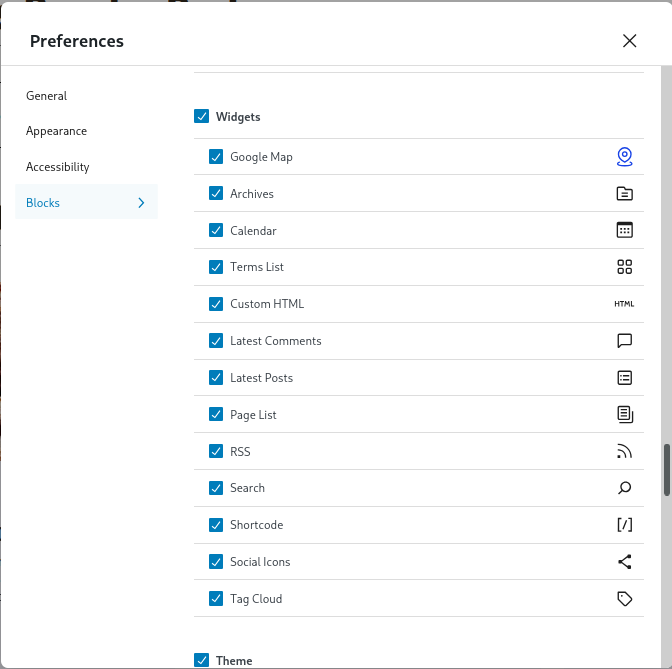
\includegraphics[width=0.75\textwidth]{images/widget-block-confusion.png}
        \end{figure}

    \item Motivo de elección del tema

    El tema seleccionado incluye la etiqueta "footer widgets" y permite replicar todas las funciones tradicionales de widgets mediante:

    \begin{itemize}
        \item Bloques nativos (ej: listas de contenido, menús).
        \item Plantillas personalizables (Appearance → Editor), donde se diseña el pie de página con elementos dinámicos.
    \end{itemize}

    Esto generó confusión inicial, ya que la documentación no siempre diferencia claramente entre widgets clásicos y su equivalencia en bloques.

    \item Recursos de referencia
        \begin{itemize}
            \item \href{https://wordpress.org/documentation/article/block-themes/#what-is-a-block-theme}{Documentación oficial sobre temas de bloques}
            \item \href{https://torquemag.io/2023/06/wordpress-widget-areas/}{Guía sobre cómo añadir áreas de widgets}
        \end{itemize}

\end{enumerate}

\subsection{Creación del widget}

Se ha intentado la creación de un widget pero no se ha conseguido mostrar en temas de bloques.
La creación del plugin sí se consiguió.

\begin{figure}[H]
    \centering
    
\includegraphics[width=0.85\textwidth]{images/custom-plugin.png}
\end{figure}


\newpage


\section{SEO, seguridad, aspectos legales y accesibilidad}

\subsection{SEO}

Después de instalar Yoast SEO se hizo la configuración inicial.

\begin{figure}[H]
    \centering
    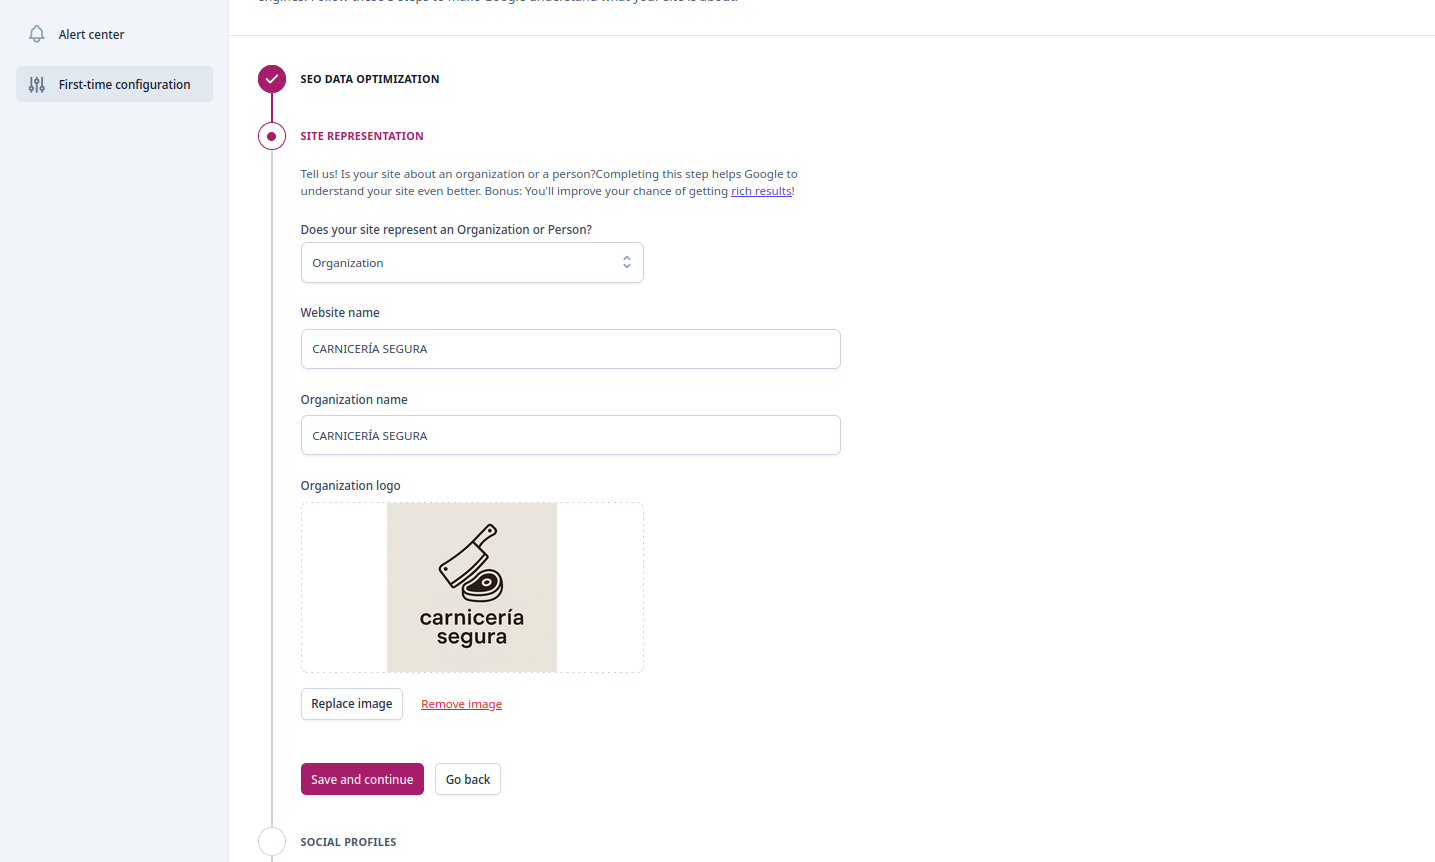
\includegraphics[width=0.85\textwidth]{images/yoast1.png}
    \caption{Configuración inicial de Yoast SEO}
\end{figure}

\subsubsection{Análisis de la página principal}

Al comienzo del proceso, el análisis de la página principal era negativo como se puede ver en la siguiente imagen.

\begin{figure}[H]
    \centering
    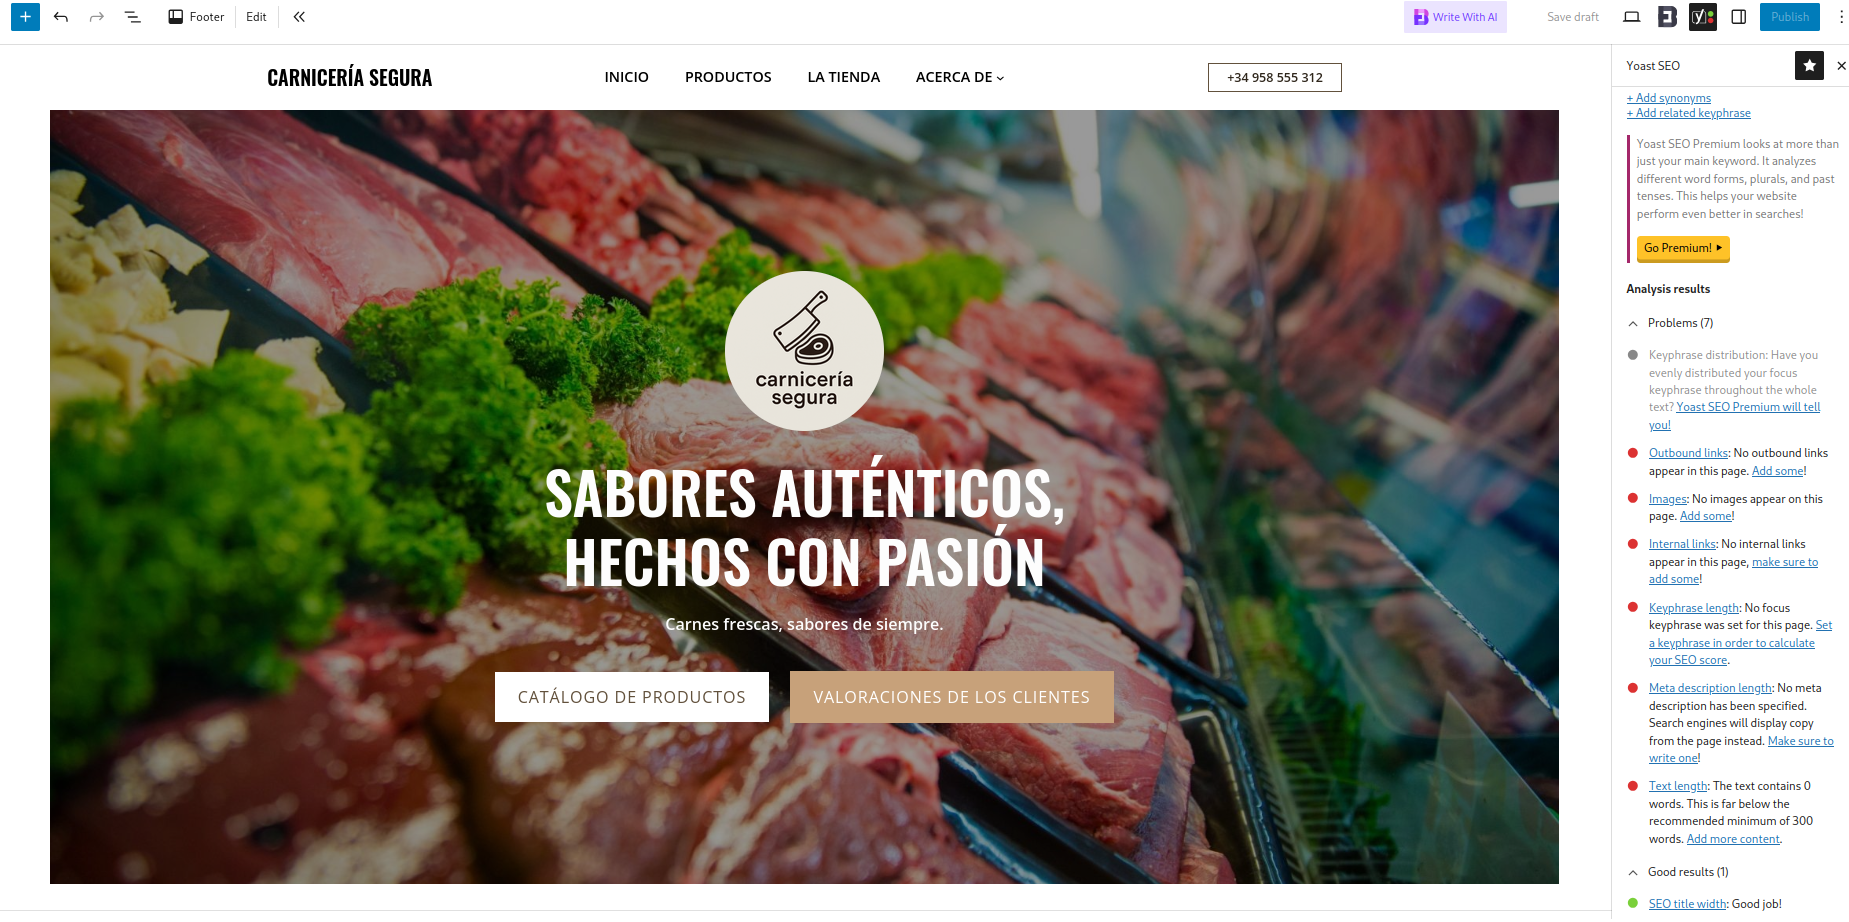
\includegraphics[width=0.85\textwidth]{images/yoastl1.png}
    \caption{Valoración inicial de Yoast SEO}
\end{figure}

Para mejorar el SEO de la página principal, he aplicado varias técnicas básicas pero efectivas. En primer lugar, añadí un título optimizado para SEO, incluyendo palabras clave relevantes como “Carnicería, carnes, embutidos, caseros” para mejorar el posicionamiento en búsquedas relacionadas. También redacté una meta descripción clara y atractiva, pensada para responder de forma directa a las intenciones de búsqueda de los usuarios.

\begin{figure}[H]
    \centering
    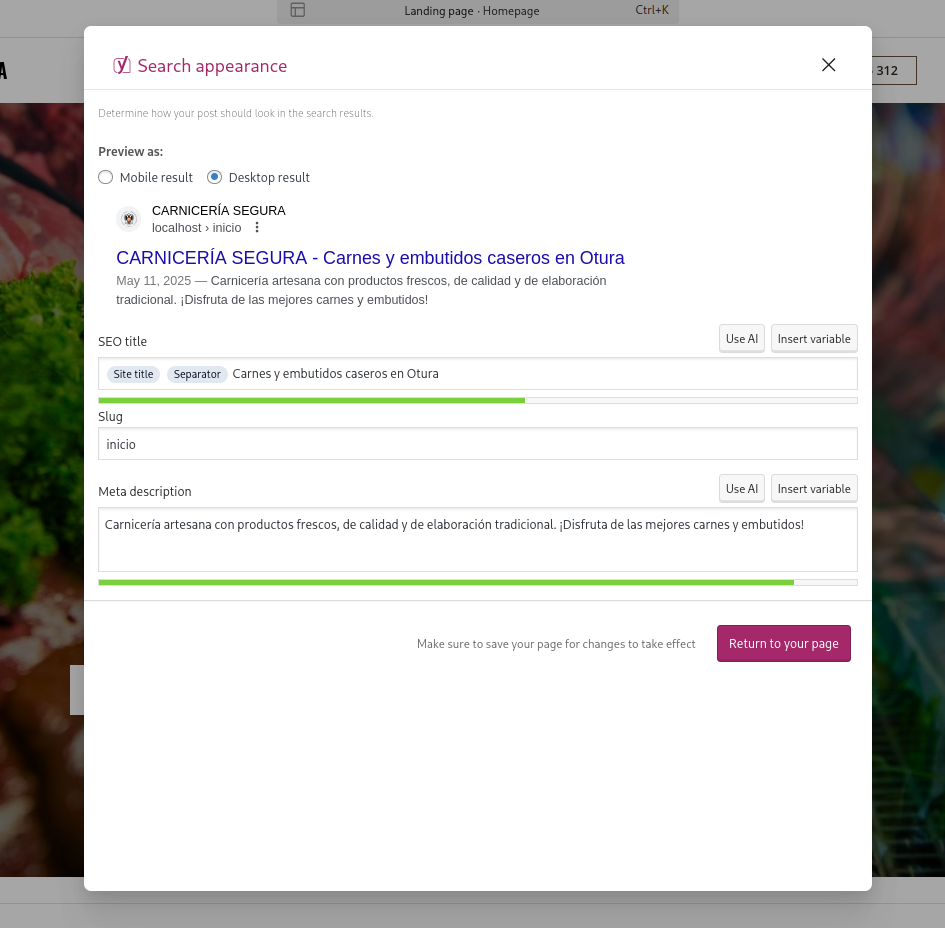
\includegraphics[width=0.85\textwidth]{images/yoastl2.png}
    \caption{Título SEO y meta descripción}
\end{figure}

Además, estructuré el contenido principal con párrafos introductorios bien definidos, que resumen la actividad y los valores del negocio de forma concisa. Para mejorar la legibilidad y cumplir con las recomendaciones de herramientas como Yoast SEO, utilicé frases más cortas y conectores que facilitan la lectura y la navegación semántica del texto.

\textgap

Asimismo, incorporé enlaces externos hacia otras páginas interesantes (comercios locales del pueblo) para mejorar la estructura interna y la experiencia de usuario. Por último, definí una palabra clave principal (keyphrase) para enfocar todo el contenido en torno a ella, evitando repeticiones excesivas y usando sinónimos cuando era necesario, manteniendo siempre la naturalidad del texto.

\textgap

Gracias a estos cambios, el contenido de la página no solo es más atractivo para los visitantes, sino también más eficiente desde el punto de vista del posicionamiento en buscadores.

\begin{figure}[H]
    \centering
    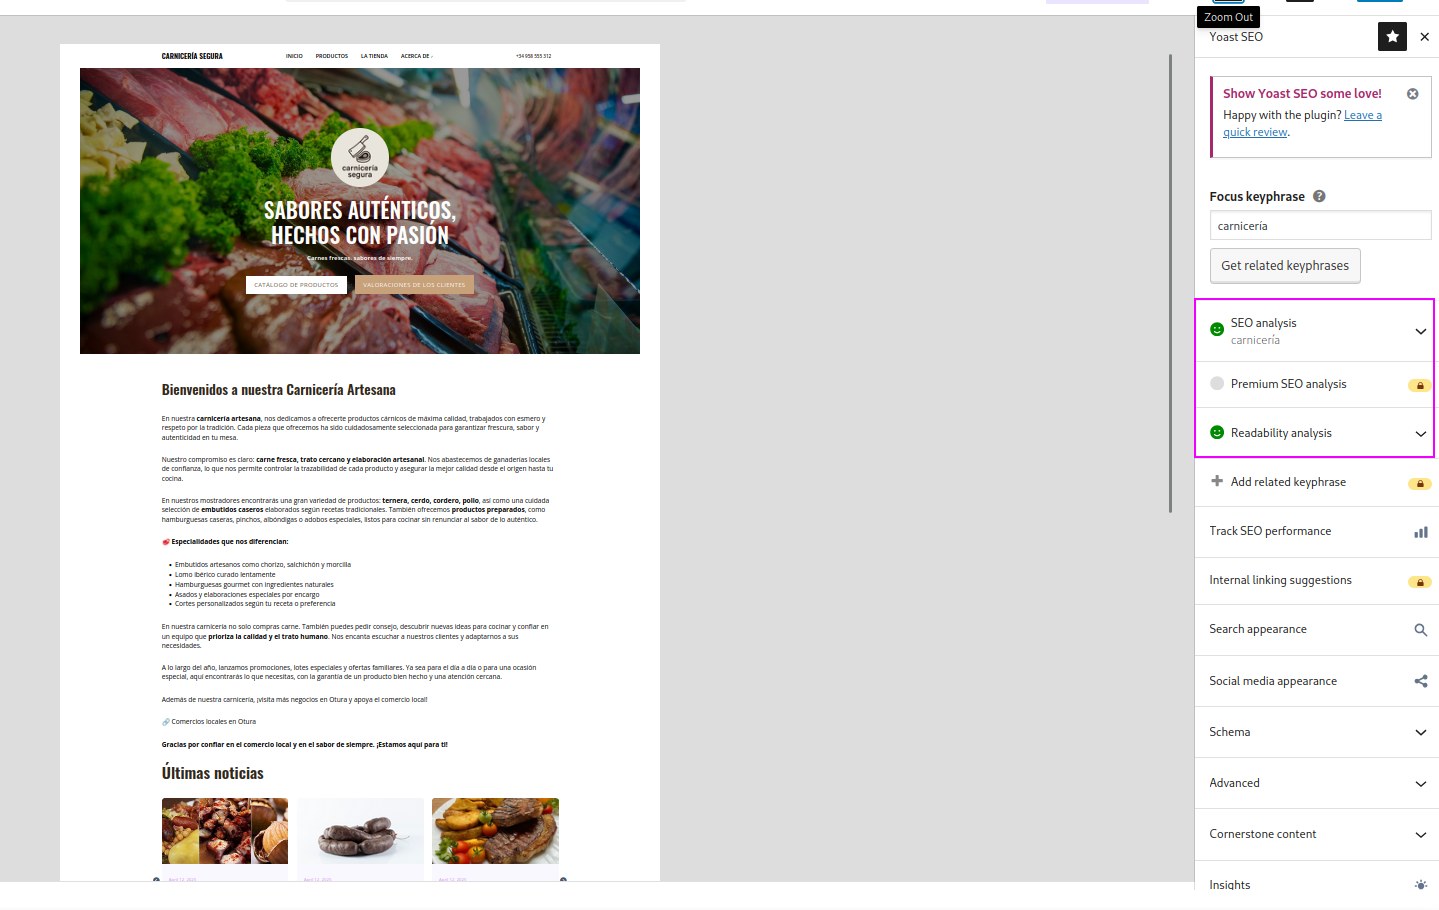
\includegraphics[width=0.85\textwidth]{images/yoastl3.png}
    \caption{Resultado final de la optimización SEO}
\end{figure}


\subsubsection{Análisis de una noticia}

Al comienzo del proceso, el análisis del contenido inicial de la noticia era negativo como se puede ver en la siguiente imagen. En ese momento, el plugin marcaba varios problemas relacionados con el posicionamiento, debido a la falta de enlaces externos e internos y la corta extensión del texto.

\begin{figure}[H]
    \centering
    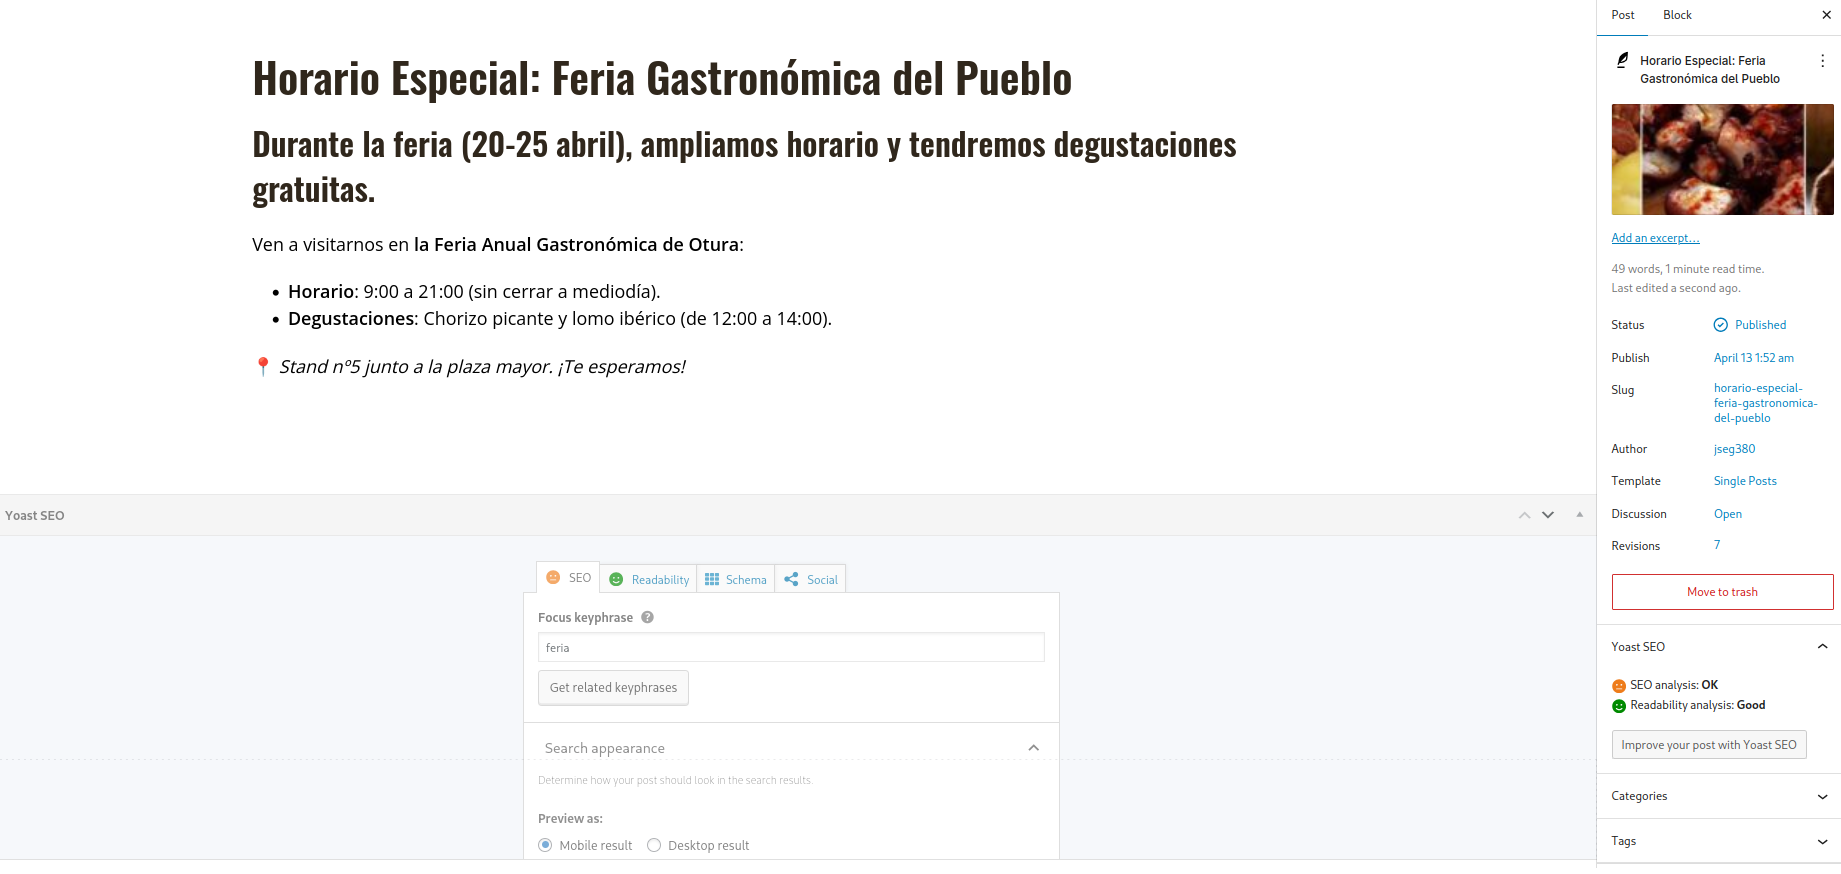
\includegraphics[width=0.85\textwidth]{images/yoast2.png}
    \caption{Configuración inicial de Yoast SEO}
\end{figure}

Para solucionarlo, reescribimos la noticia para que su extensión fuera mayor a 300 palabras, añadiendo enlaces externos relevantes. Pero ahora el plugin indicaba que el contenido era difícil de leer, con frases largas y complejas que dificultaban la comprensión.

\begin{figure}[H]
    \centering
    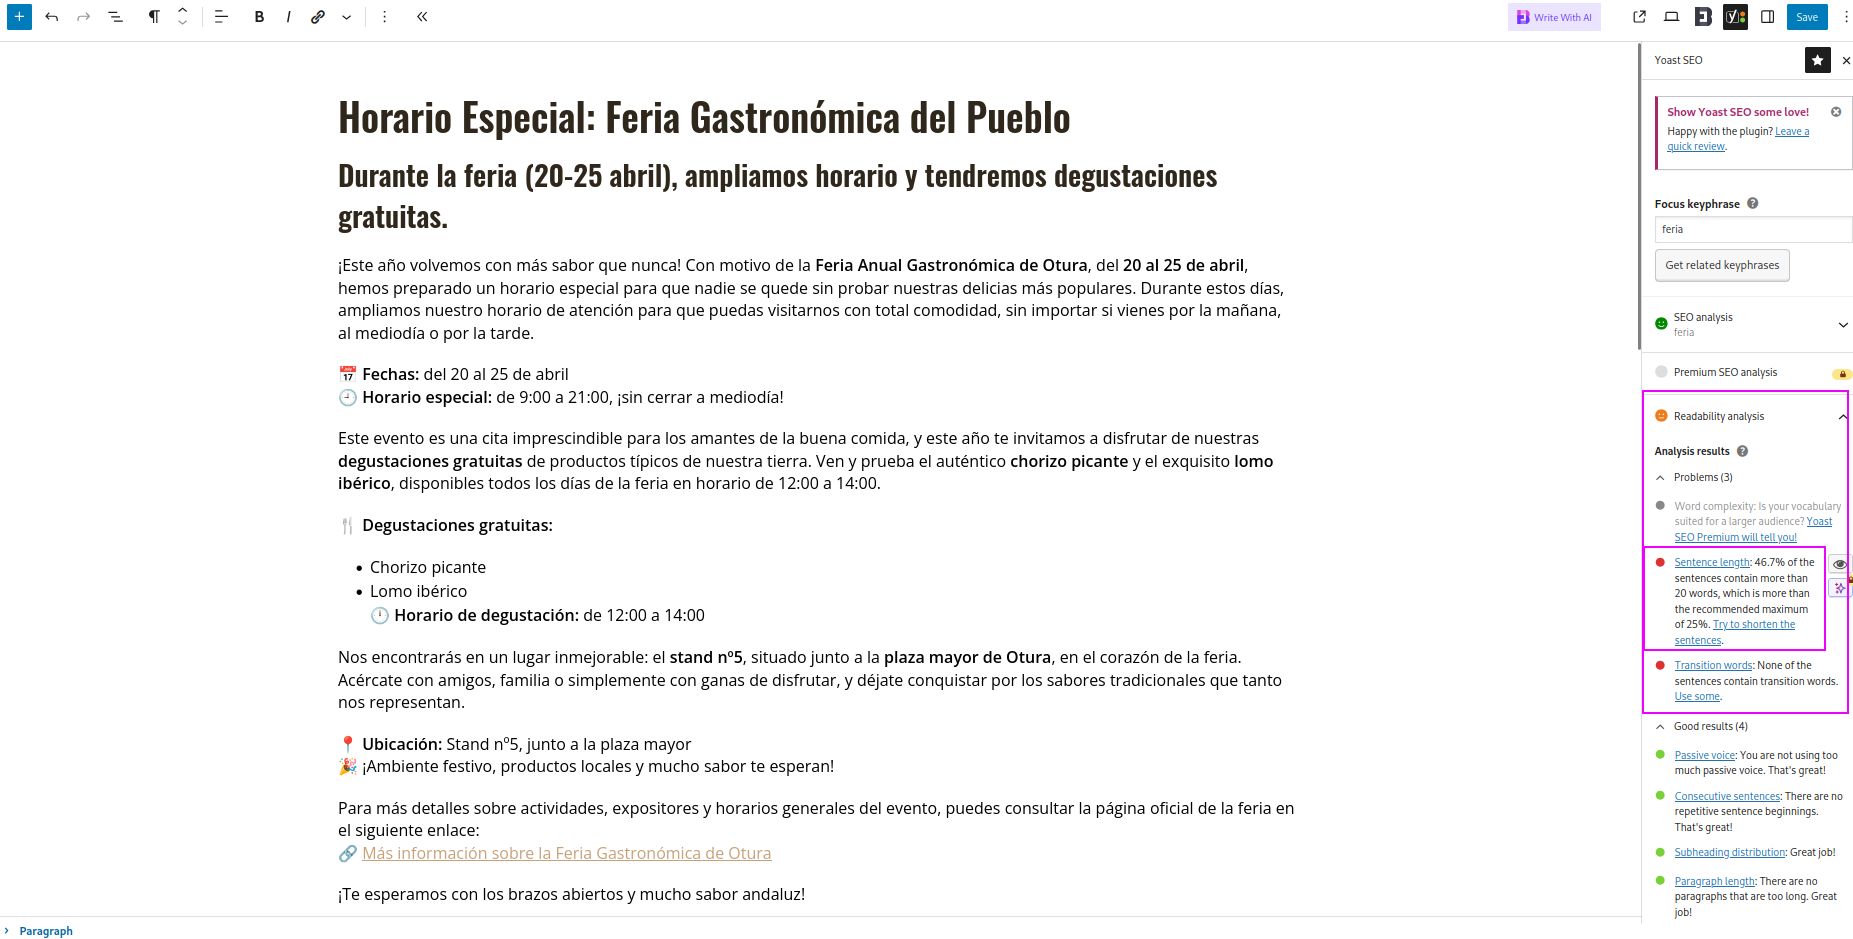
\includegraphics[width=0.85\textwidth]{images/yoast3.png}
    \caption{Configuración inicial de Yoast SEO}
\end{figure}

Tras analizar las palabras de transición y ver que no correspondían en este tipo de noticia, los esfuerzos se centraron en mejorar la legibilidad de las frases, reduciendo su tamaño y aumentando su cantidad a cambio.

\begin{figure}[H]
    \centering
    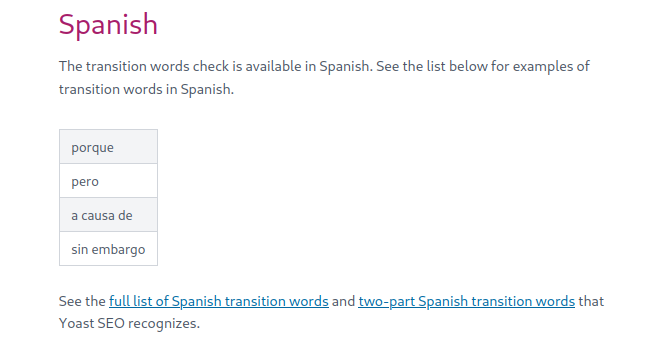
\includegraphics[width=0.85\textwidth]{images/yoast31.png}
    \caption{Palabras de transición según Yoast SEO}
\end{figure}

Para solucionarlo, reescribimos el contenido con frases más cortas y directas, asegurándonos de que la mayoría no superaran las 20 palabras. Además, añadimos conectores para facilitar la lectura y mejorar la coherencia entre párrafos.

 \begin{figure}[H]
    \centering
    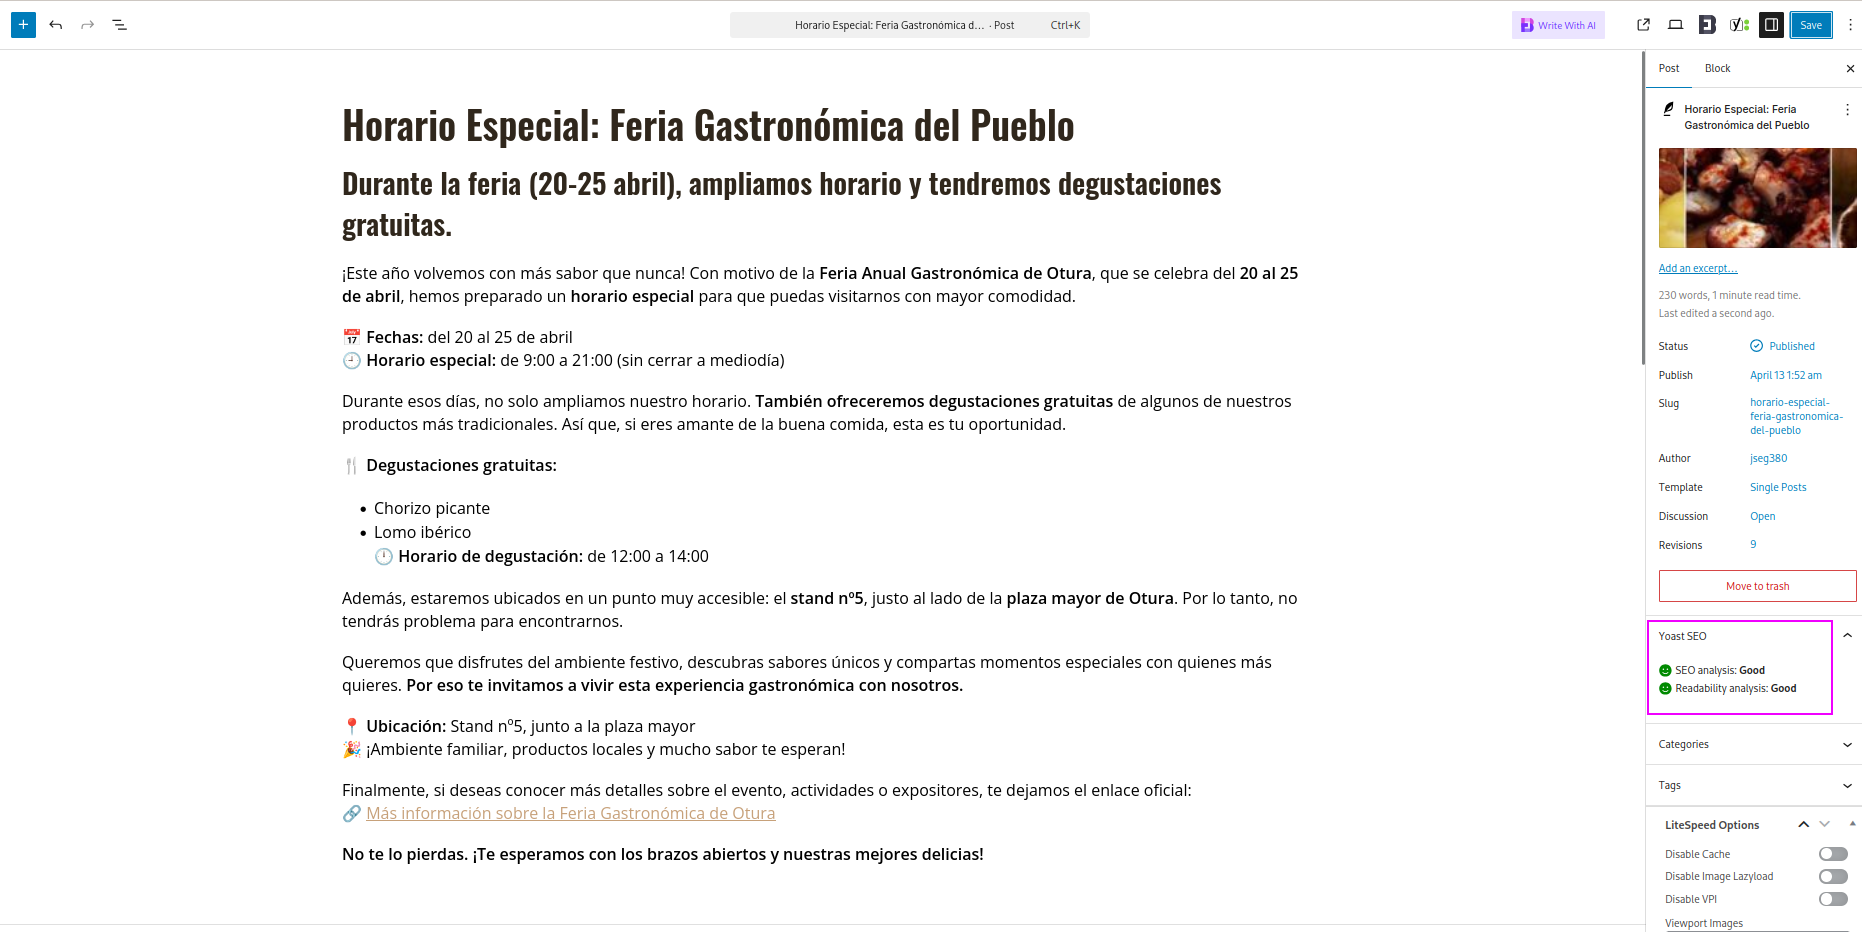
\includegraphics[width=0.85\textwidth]{images/yoast4.png}
    \caption{Buena valoración de Yoast SEO}
\end{figure}

\subsection{Seguridad}

Al instalar Wordfence, este parece tener una funcionalidad para ``auto-configurarse'', y tiene sentido ya que la mayoría de las funcionalidades que ofrece parecen estar detrás de un ``paywall''.

\begin{figure}[H]
    \centering
    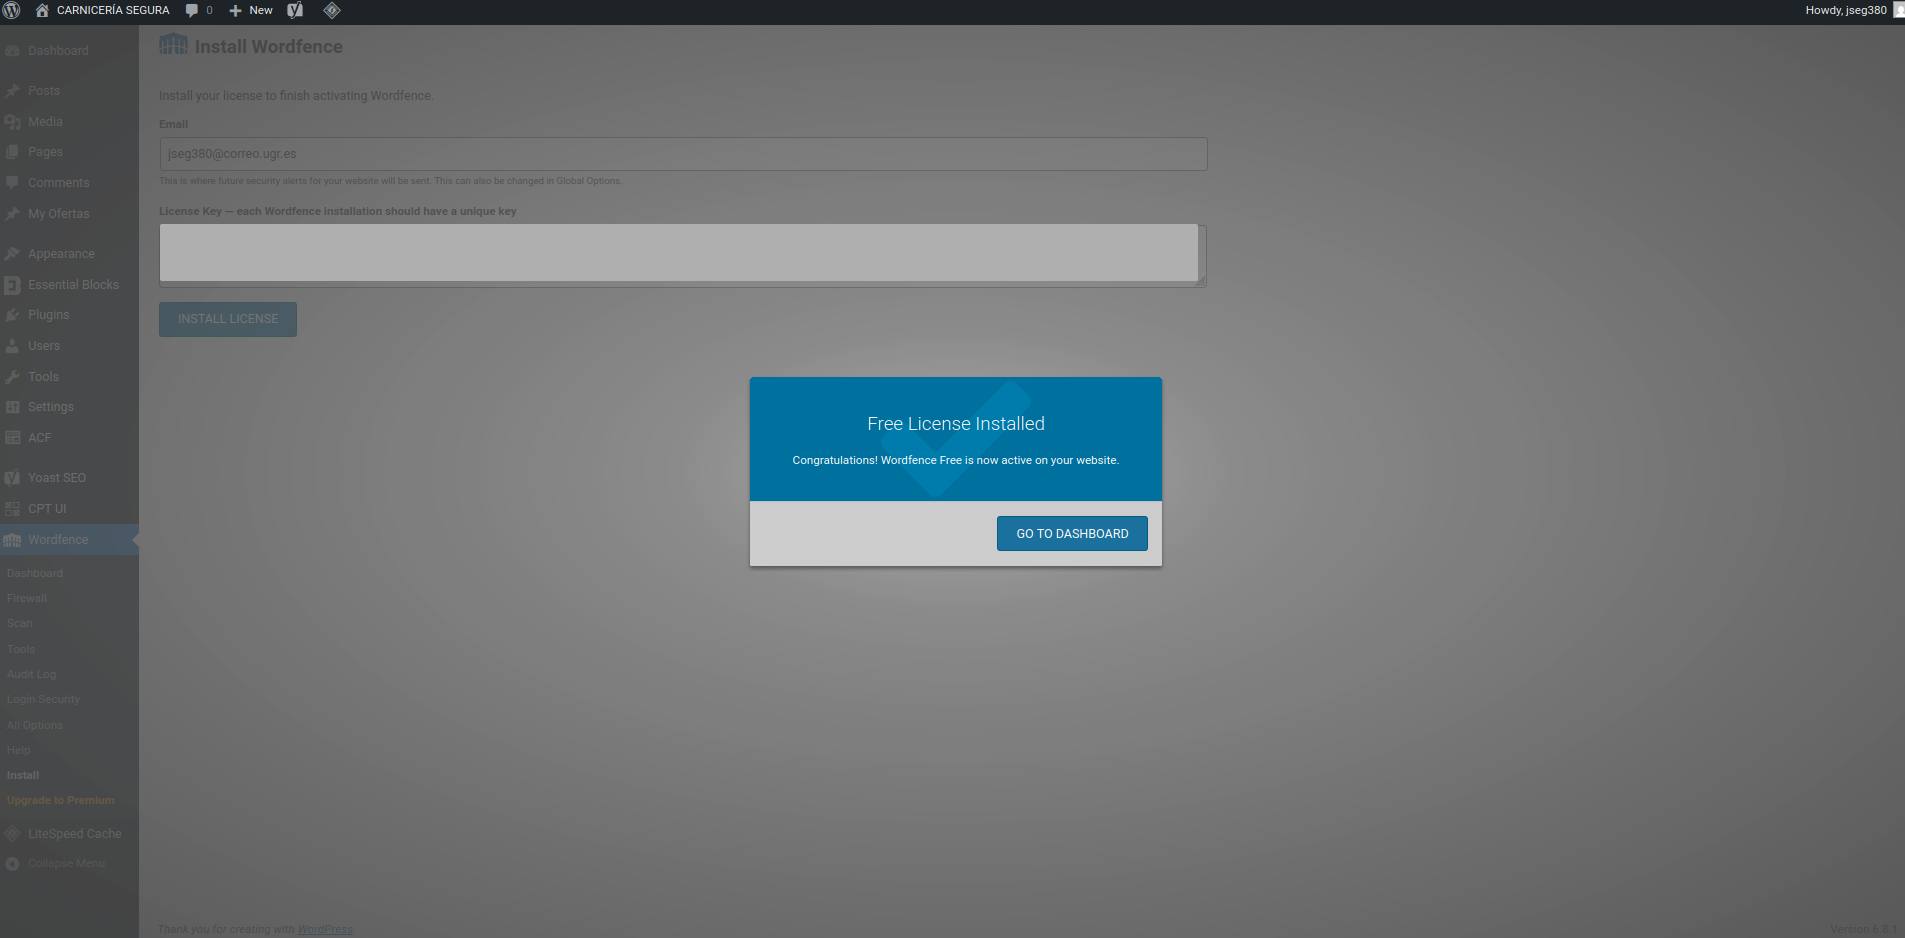
\includegraphics[width=0.85\textwidth]{images/wordfence1.png}
    \caption{Instalación de la versión gratuita de Wordfence}
\end{figure}

\begin{figure}[H]
    \centering
    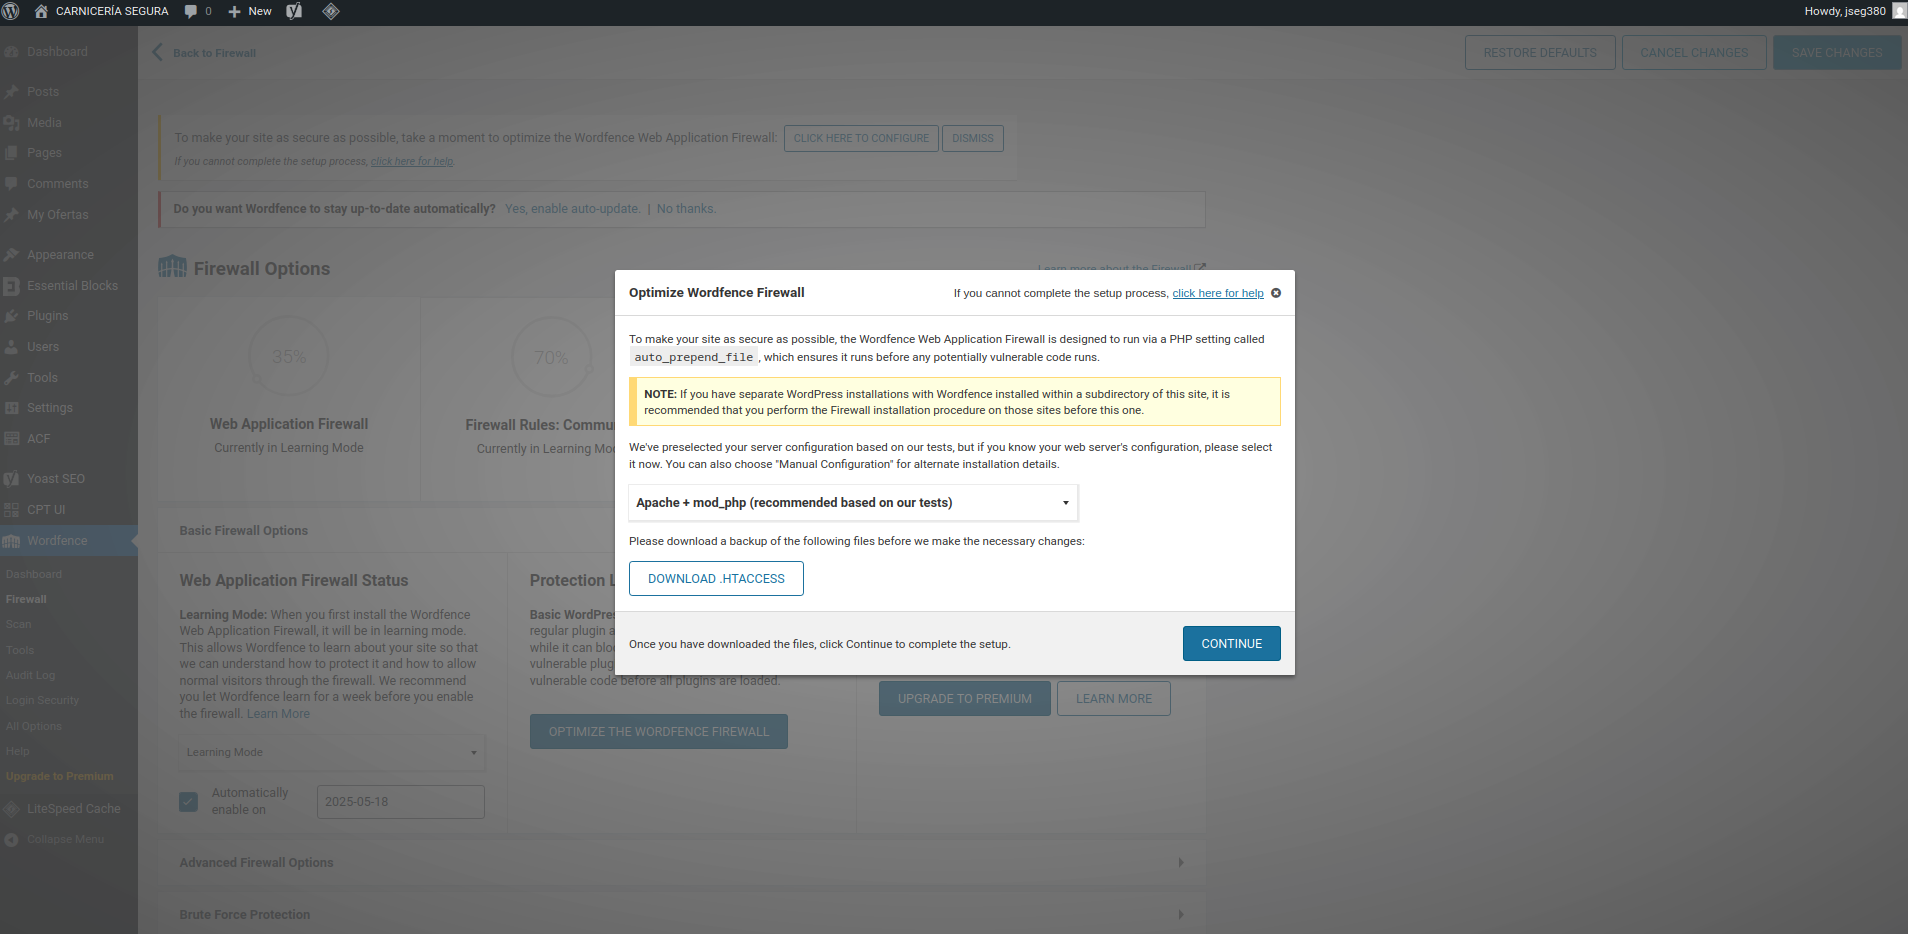
\includegraphics[width=0.85\textwidth]{images/wordfence2.png}
    \caption{Optmización de la configuración de Wordfence}
\end{figure}

\begin{figure}[H]
    \centering
    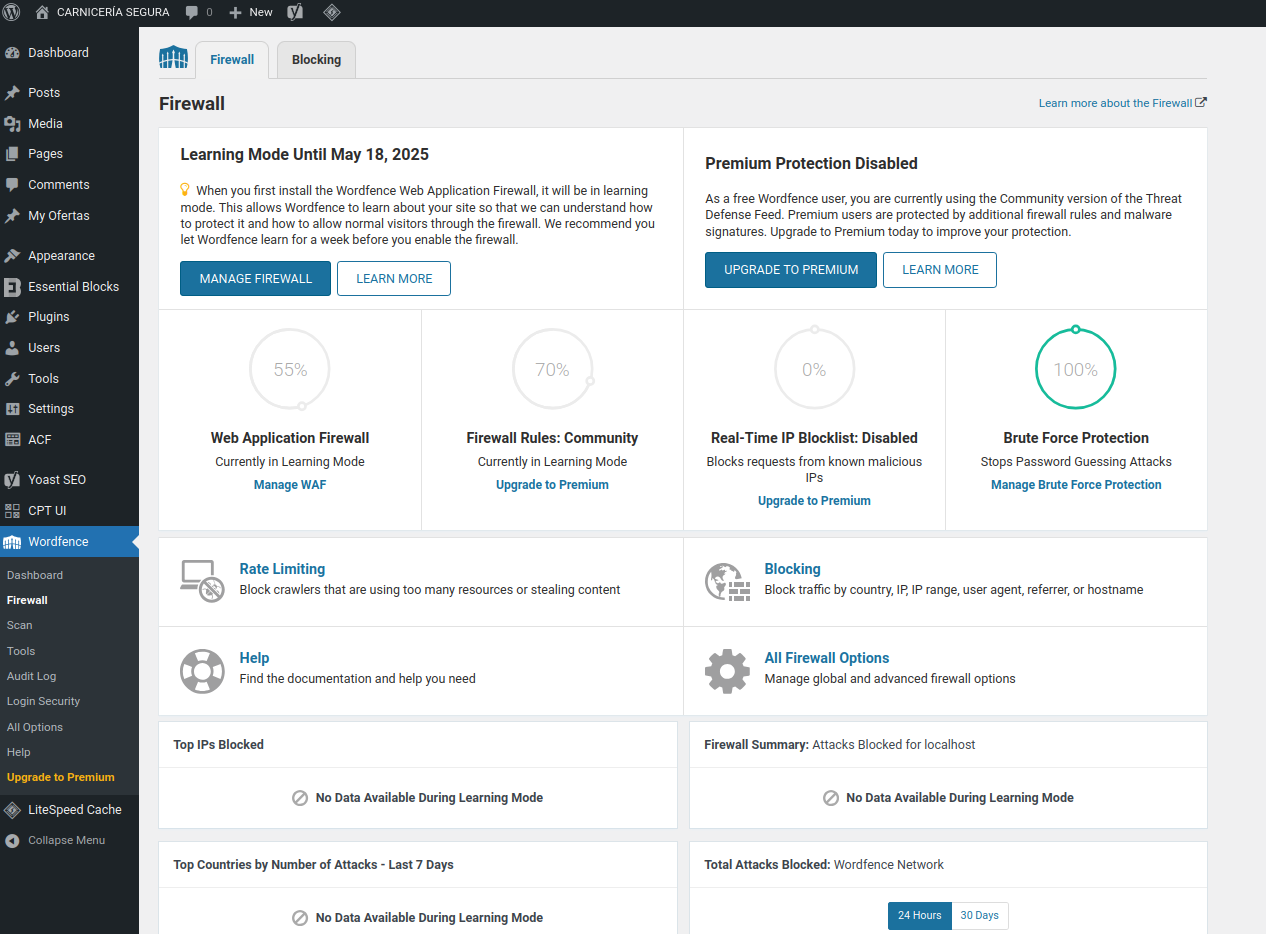
\includegraphics[width=0.85\textwidth]{images/wordfence3.png}
    \caption{Estado actual}
\end{figure}

\subsection{Aspectos legales}

Ya que la página se está ejecutando en local por el momento, no se han podido implementar los aspectos legales que se deberían tener en cuenta al poner la página en producción, especialmente aquellos relativos a cookies, aún así se ha hecho un borrador de cómo podría quedar:

\begin{figure}[H]
    \centering
    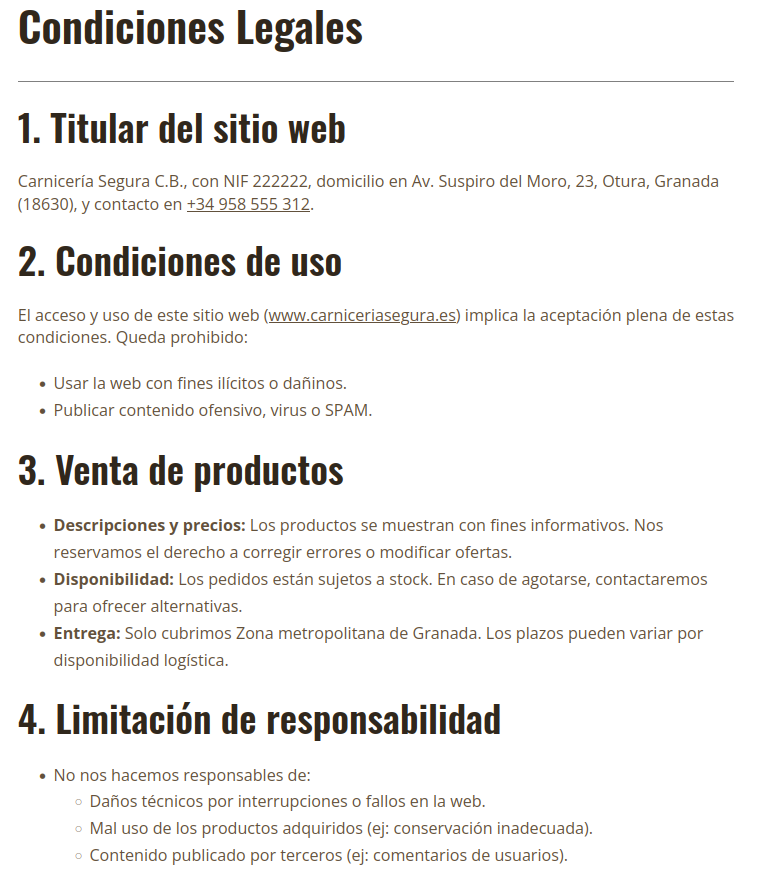
\includegraphics[width=0.85\textwidth]{images/legal1.png}
    \caption{Aviso legal}
\end{figure}

\begin{figure}[H]
    \centering
    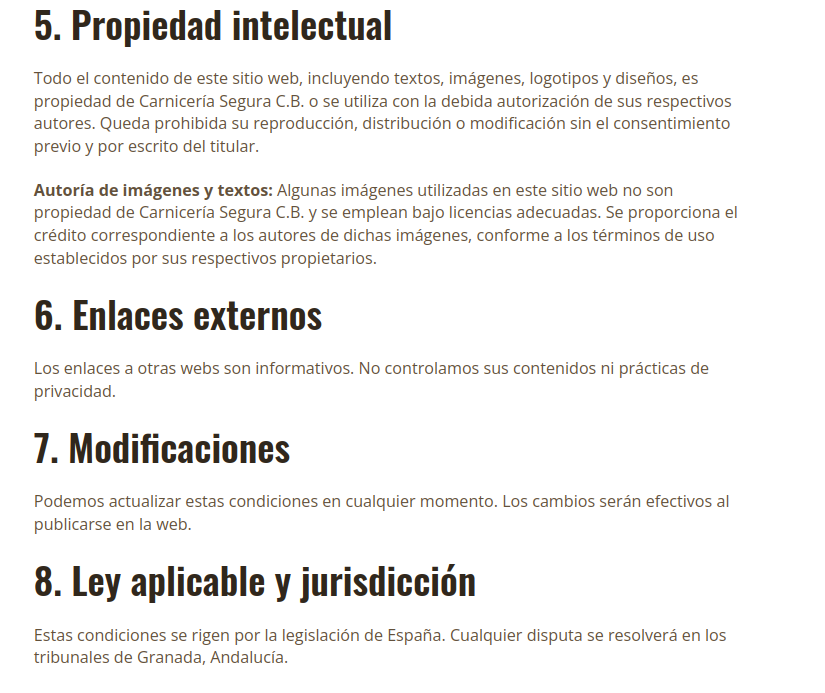
\includegraphics[width=0.85\textwidth]{images/legal2.png}
    \caption{Aviso legal}
\end{figure}

\begin{figure}[H]
    \centering
    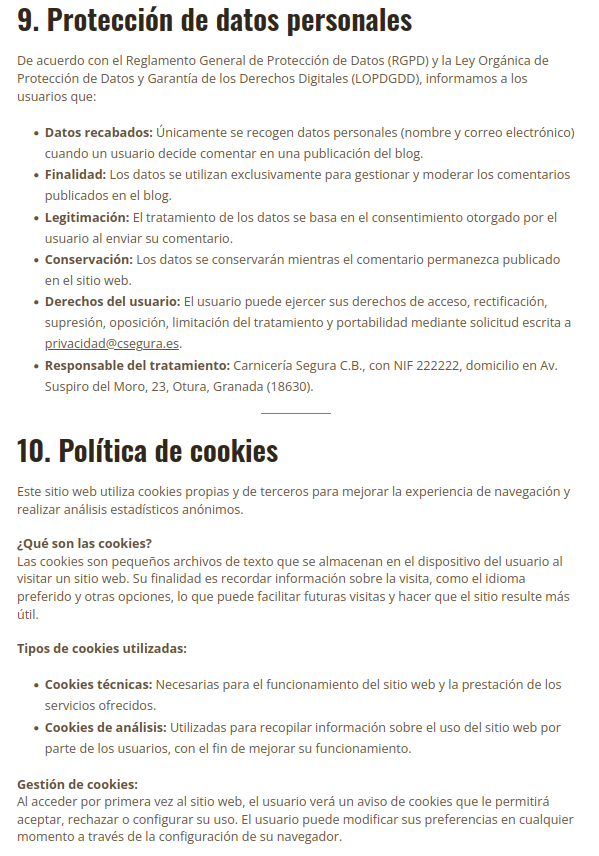
\includegraphics[width=0.85\textwidth]{images/legal3.png}
    \caption{Aviso legal}
\end{figure}

\subsection{Accesibilidad}

\subsubsection{Informe de Accesibilidad Funcional – Página Principal}

\begin{enumerate}
    \item Idioma del contenido

    El contenido de la página está íntegramente en español, pero el idioma declarado en la estructura HTML es inglés (lang="en-US"). Esto puede provocar que los lectores de pantalla interpreten erróneamente la pronunciación del texto, afectando negativamente a la comprensión auditiva por parte de usuarios con discapacidad visual.

    \item Estructura de encabezados y contenido

    La jerarquía de encabezados está presente y es funcional, facilitando la orientación de usuarios que utilizan tecnologías de asistencia. El sitio presenta contenido distribuido en bloques claramente diferenciados, lo cual mejora la legibilidad.

    \item Imágenes y contenido visual

    Algunas imágenes incluidas en la página principal no disponen de texto alternativo (alt). Esto impide que los lectores de pantalla transmitan información visual esencial a los usuarios con discapacidad visual. Las imágenes decorativas tampoco están marcadas correctamente como tal (alt=""), lo que introduce ruido informativo innecesario.

    \item Saltar al contenido principal

    Se incluye un enlace "Saltar al contenido" visible solo para lectores de pantalla o al usar el teclado, lo cual es adecuado para facilitar la navegación directa al contenido relevante.

    \item Carrusel de entradas recientes

    Se observa un componente tipo carrusel de posts. No se puede controlar mediante teclado. Esto representa un punto de accesibilidad crítica, ya que los carruseles mal implementados son una barrera frecuente para usuarios con discapacidad visual, cognitiva o movilidad reducida.

    \item Compatibilidad con tecnologías de asistencia

    No se incluyen atributos ARIA (aria-*) observables en la estructura actual. Si bien WordPress no los genera automáticamente, algunos temas o plugins pueden incluirlos. En este caso, no se evidencia su presencia, lo cual limita la capacidad de interpretación semántica por parte de lectores de pantalla.

\end{enumerate}


\subsubsection{Informe de Accesibilidad Funcional – Página Interna: ``La Tienda''}

\begin{enumerate}
    \item Contenido principal

    La página presenta un contenido conciso, dividido en tres secciones claramente identificables:

    \begin{itemize}
        \item Introducción institucional (“Tradición carnicera desde 1983 en Otura”).

        \item Horario de apertura al público.

        \item Dirección física del establecimiento.
    \end{itemize}

    El contenido es estático, claro y fácil de leer. No se utilizan estructuras complejas ni elementos interactivos adicionales.

    \item Jerarquía de la información

    La información está organizada en bloques lógicos, con encabezados y separaciones visuales adecuadas para facilitar la comprensión. Dado que el contenido es breve, no se detectan problemas funcionales relacionados con la estructura de encabezados o navegación interna.

    \item Accesibilidad del mapa incrustado

    La página incluye un mapa embebido de Google Maps que ha sido verificado como navegable mediante teclado. El enfoque por tabulador permite acceder a los controles del mapa, como zoom y vista de mapa/satélite, lo cual representa una buena práctica de accesibilidad para usuarios que no usan ratón.

    \item Encabezado y pie de página

    Se heredan del sitio principal. Como se detalla en el informe correspondiente, el menú de navegación es funcional y navegable con teclado. También se conserva el enlace de “saltar al contenido”, lo que facilita el acceso directo al área principal de la página.

    \item Imágenes y elementos visuales

    En esta página no se incluyen imágenes decorativas ni informativas, por lo que no se presentan problemas relacionados con atributos alt o descripciones alternativas.

    \item Ausencia de formularios y widgets

    La página no contiene formularios, carruseles, reproductores multimedia ni otros elementos interactivos complejos que puedan representar barreras de accesibilidad. Esto reduce significativamente el riesgo de problemas funcionales para personas con discapacidad visual, motora o cognitiva.
\end{enumerate}

\end{document}
